\section{Análisis de Estabilidad HNAF}

\subsection{Configuración del Experimento}
Fecha: 2025-08-08 09:01:03\\Modelo: models/hnaf_model_20250808_021624.pt\\Condiciones iniciales: 8\\Pasos de simulación: 200

\subsection{Trayectorias de Estado}
La Figura \ref{fig:trajectories} muestra la evolución temporal de los estados del sistema.

\begin{figure}[h]
\centering
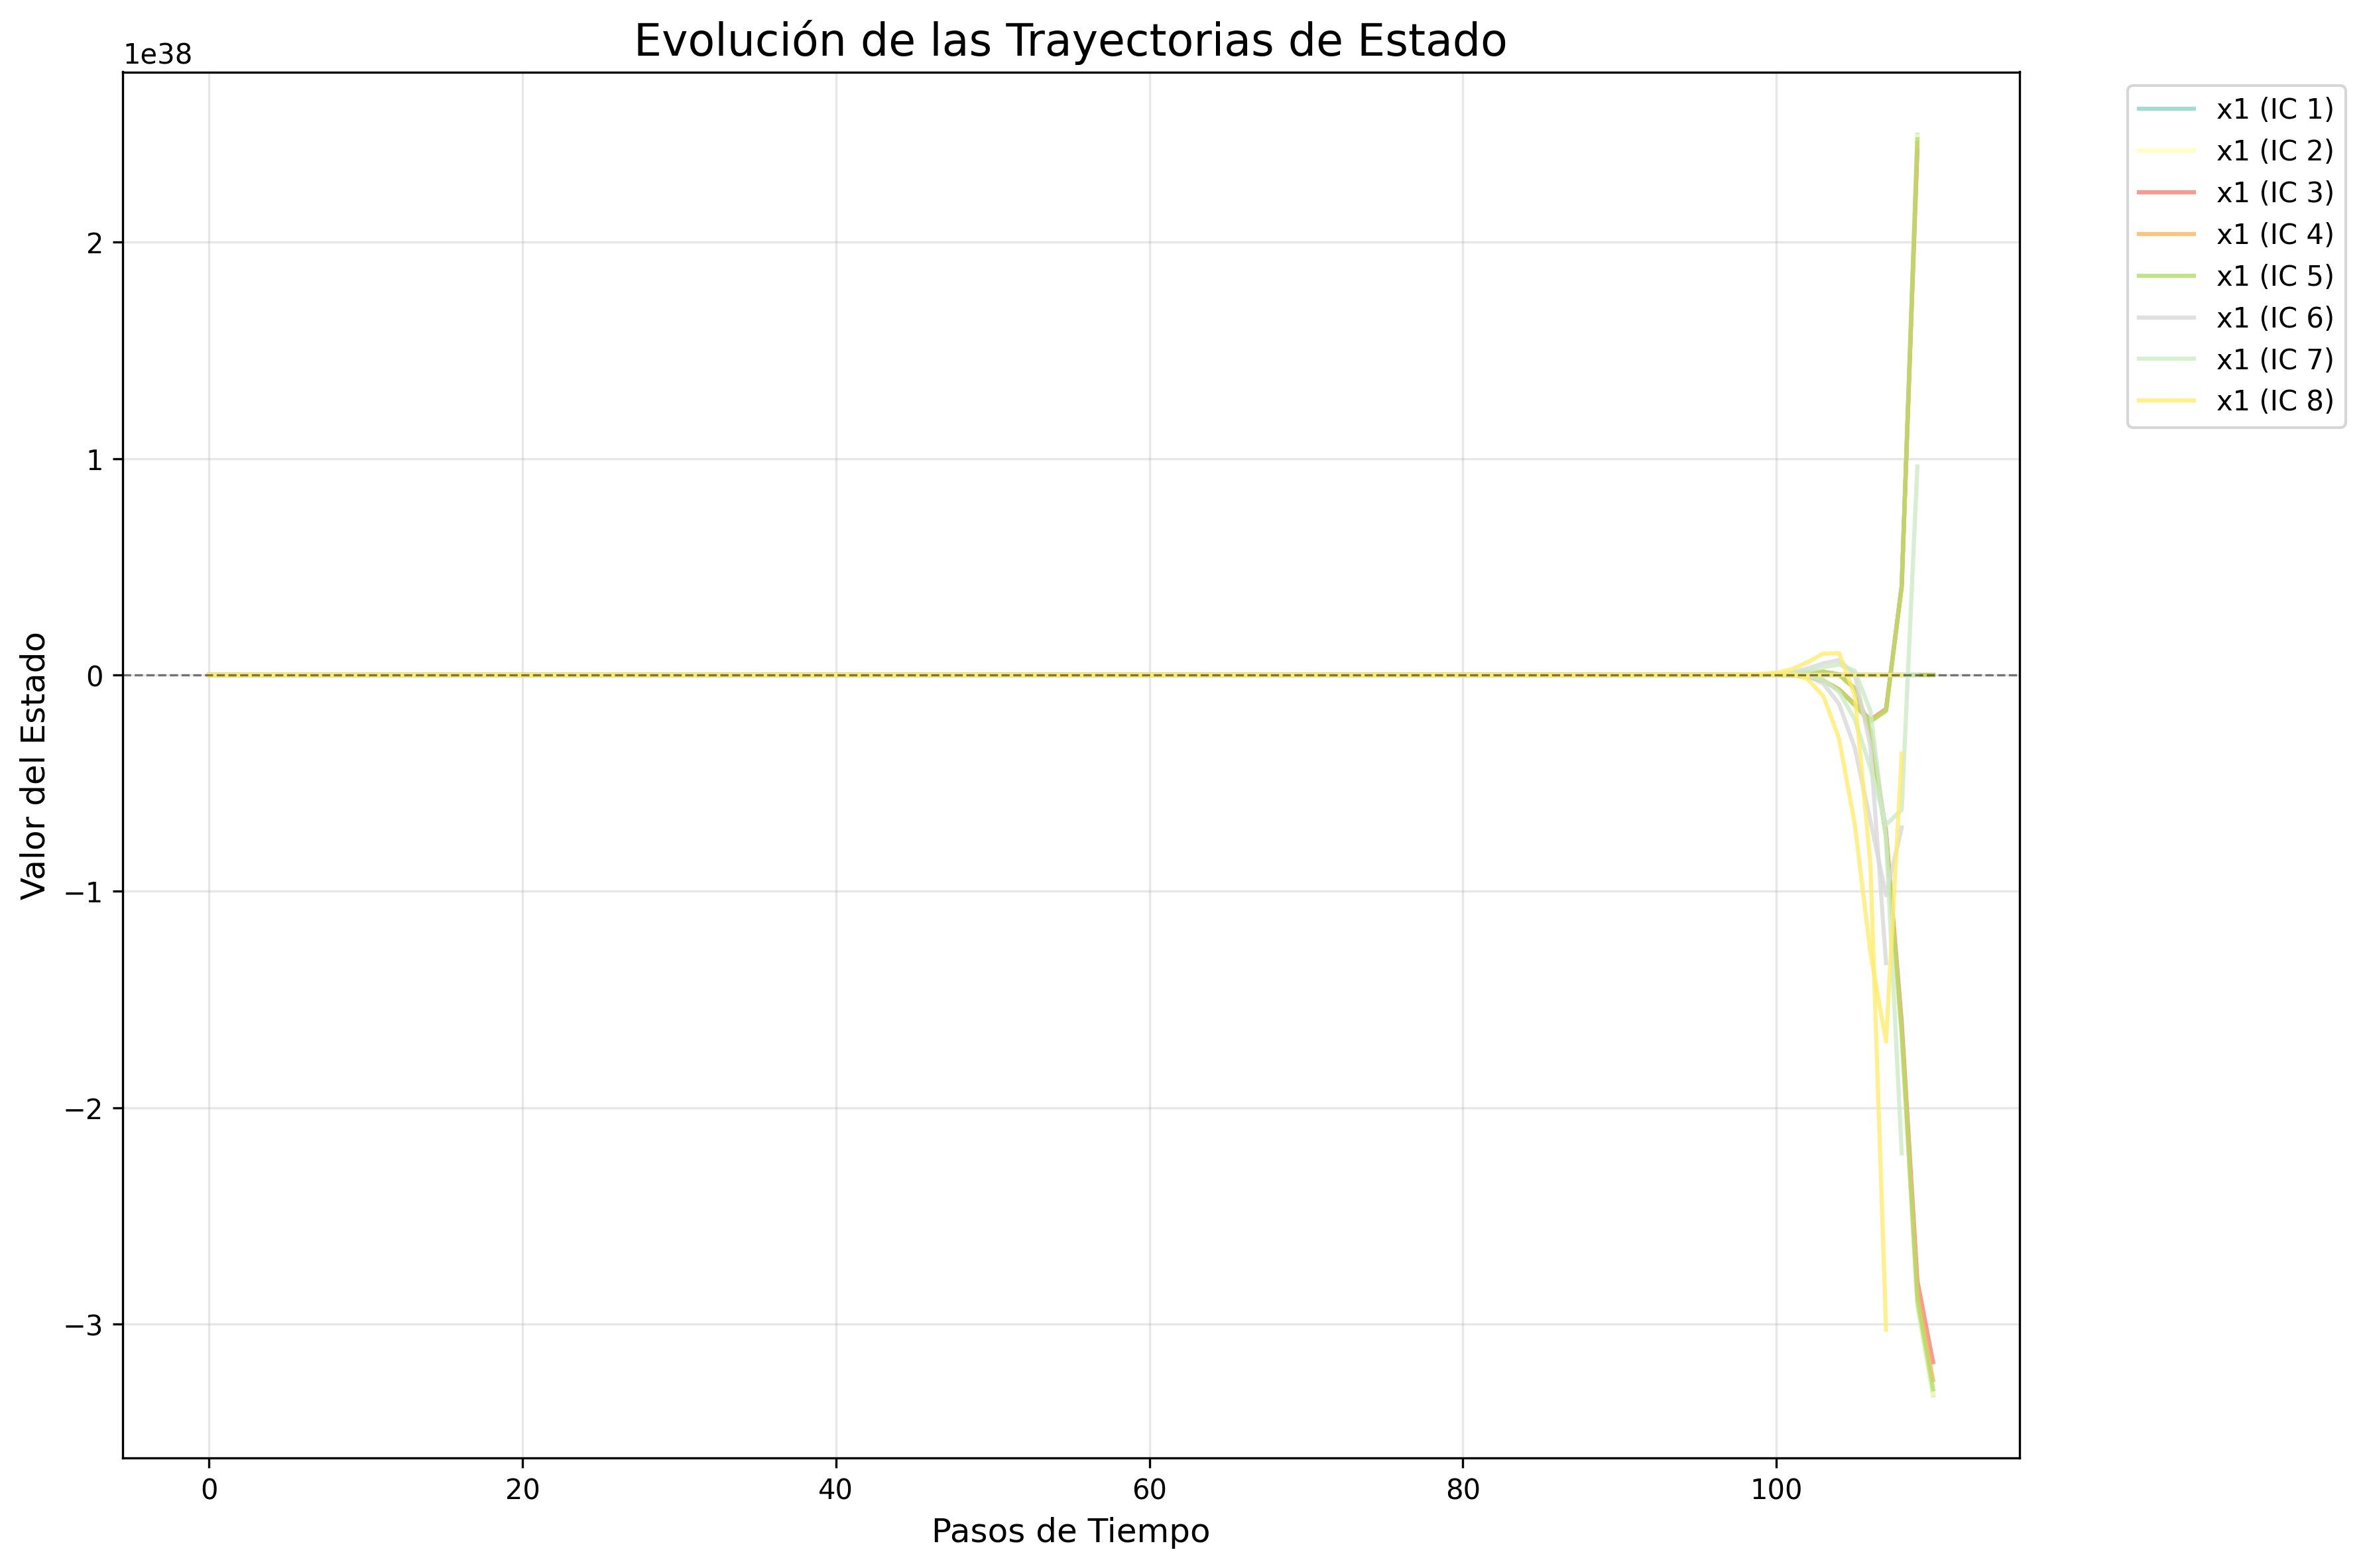
\includegraphics[width=0.8\textwidth]{plot_trajectories.png}
\caption{Trayectorias de estado para diferentes condiciones iniciales}
\label{fig:trajectories}
\end{figure}

\subsection{Ley de Conmutación}
La Figura \ref{fig:switching} ilustra la ley de conmutación aprendida.

\begin{figure}[h]
\centering
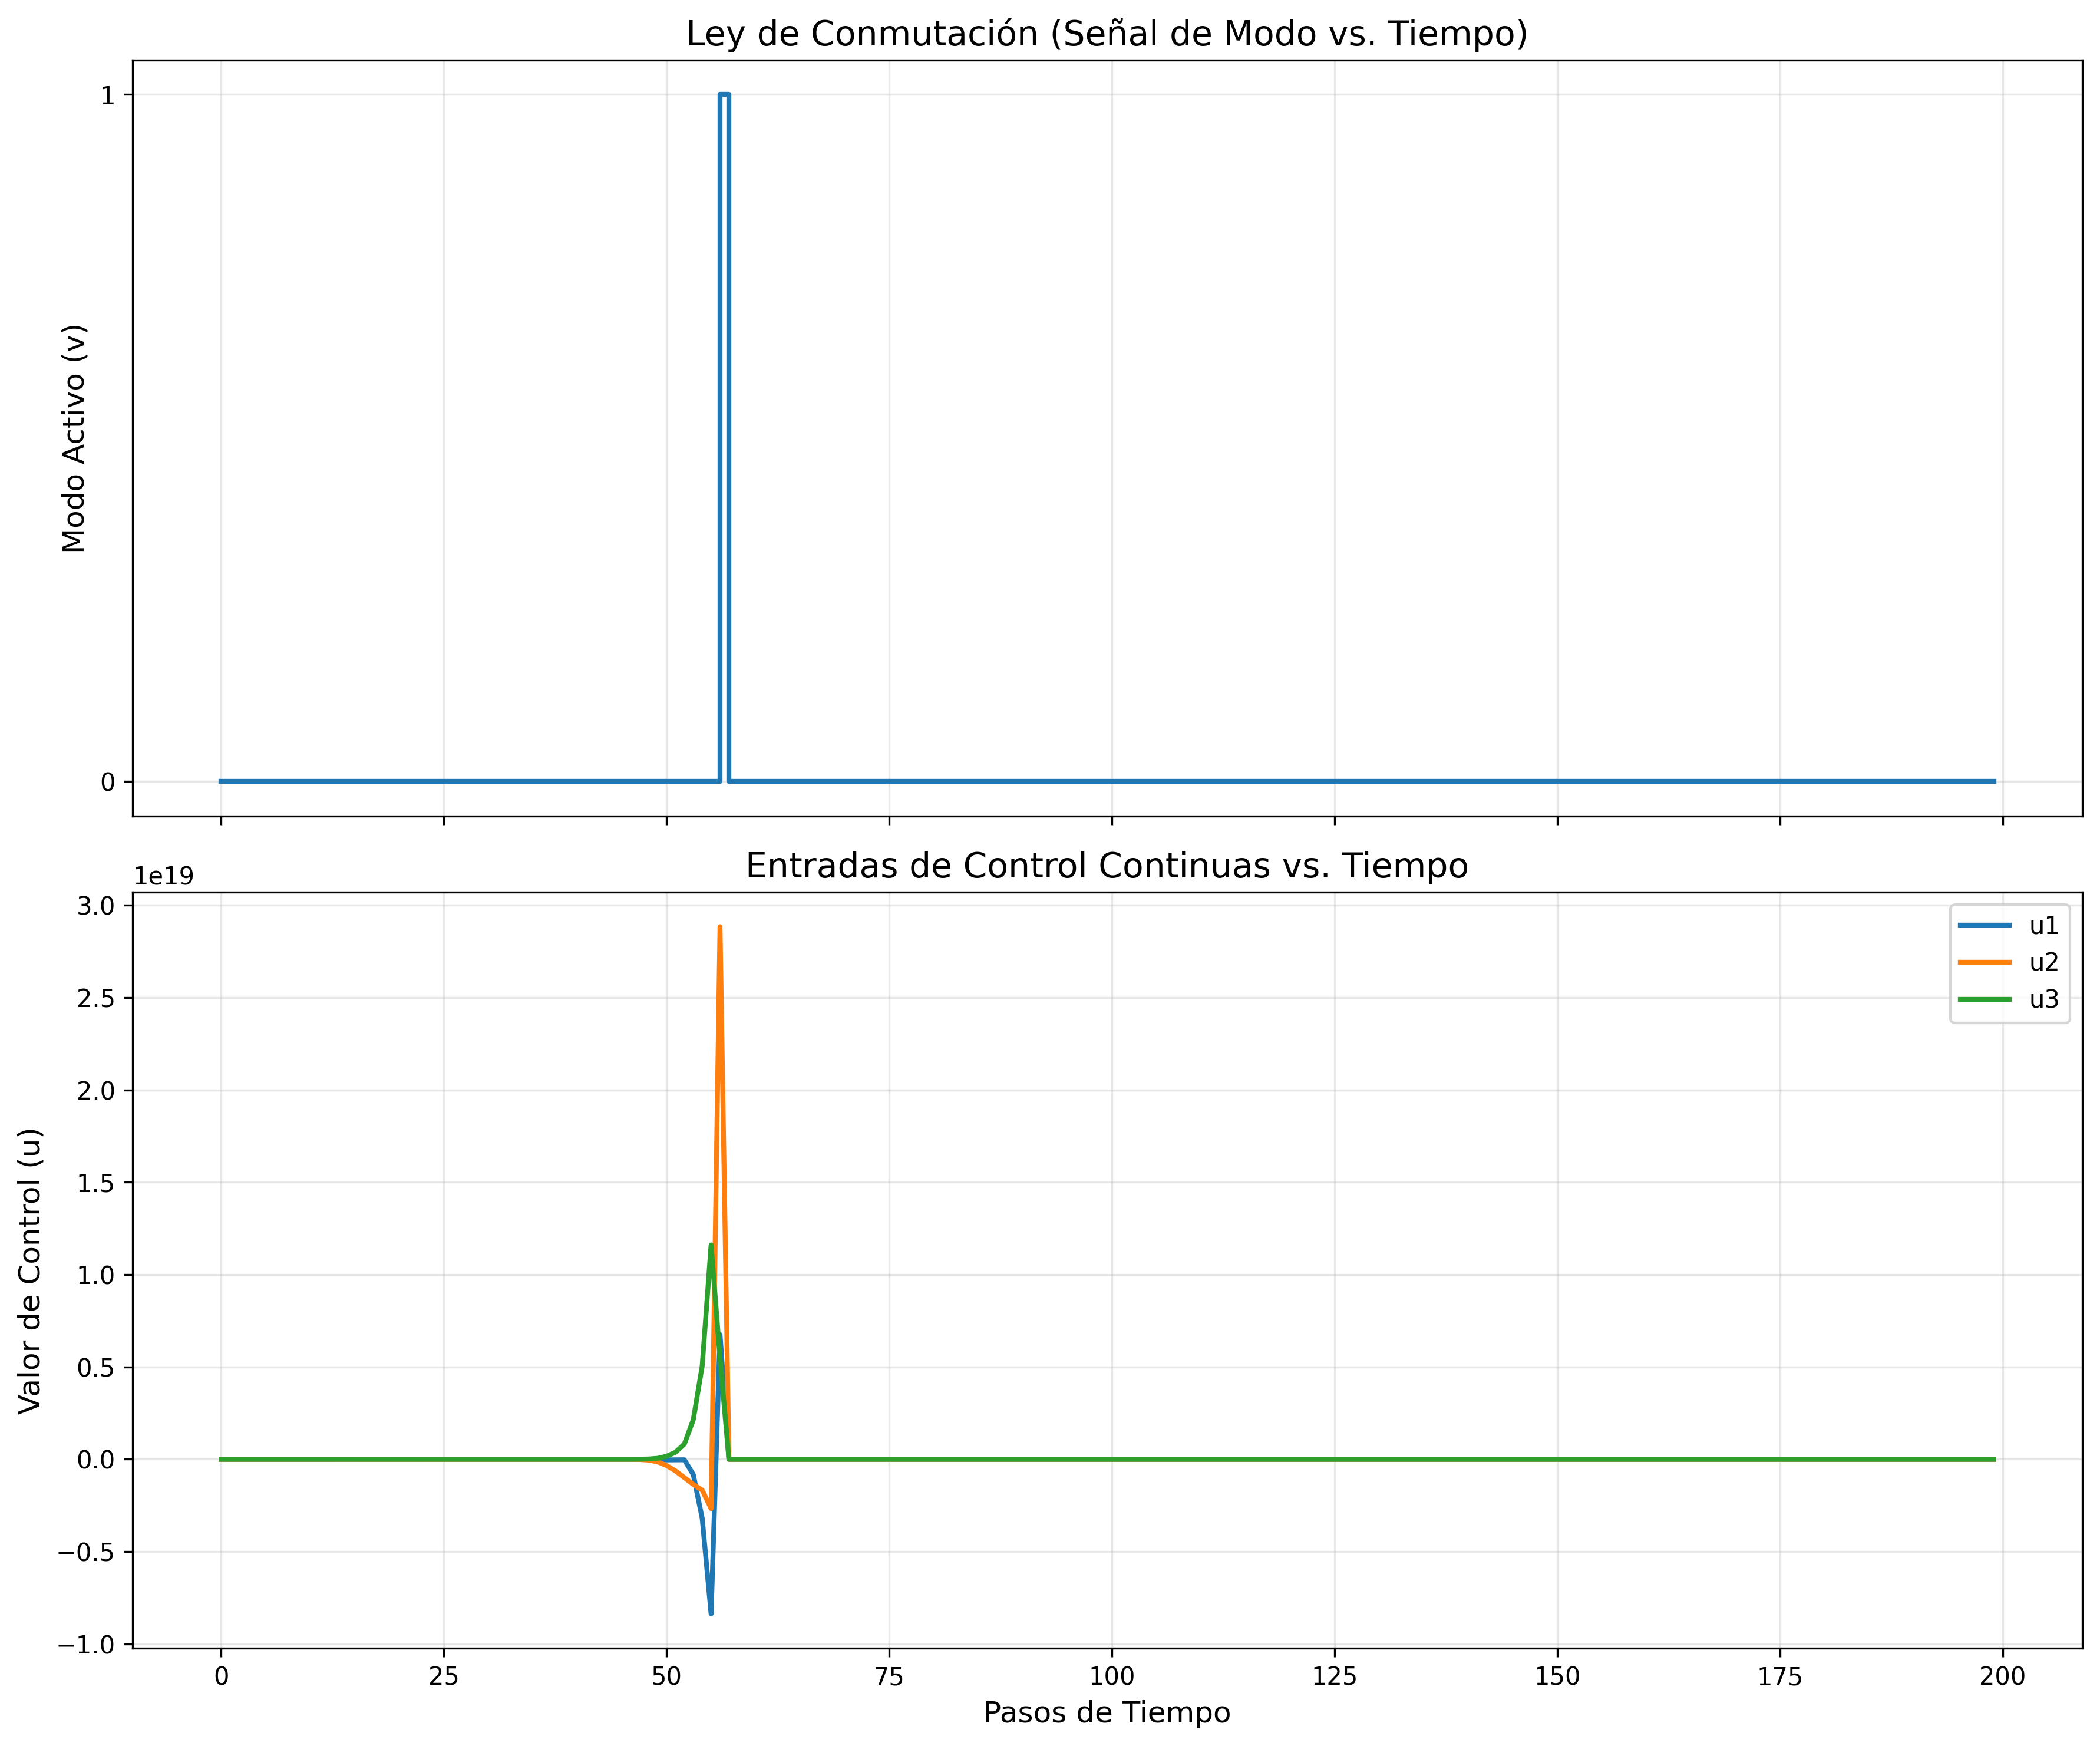
\includegraphics[width=0.8\textwidth]{plot_switching_signal.png}
\caption{Ley de conmutación y entradas de control}
\label{fig:switching}
\end{figure}

